\subsection{Line Detection}

The detection of field lines is approached in a completely different manner to that of other Objects. When searching for objects, sections of a specific colour are joined together to form a blob. While this works well for most objects, white causes problems due to its abundance in the image and hence is normally ignored. Also the thin nature of lines, and the robot's low Point Of View, makes missing pixels very common within the classified image. Finally the storing of blobs, as a square which bounds the entire object, does not store enough important information about the line.

To over come these issues the detection of lines is based around the two unique features that field lines have; their long thin length and their green-white-green transitions. Using these two details the image can be sparsely searched, since the search line does not need to find every point of the line, just enough to re-create the line. Also the transition information allows many white pixels to be thrown out early in the detection process, thereby reducing the over all load on the processor. This reliance on points and not the entire line also allows the lines to be partially hidden behind another object without effecting their detection.

With these factors in mind, the image can now be efficiently searched in the following steps;
\begin{itemize}

\item The image is searched using a horizontal and vertical search grid. The search is restricted to the area in the image below the horizon line and picks out points of sharp contrast which have green-white then white-green transitions. These points are recorded in an array for later use.

\item The found points are then checked against each other to form possible lines. Once candidates are found, more points are checked and added until a line is formed. All checks on the lines at this stage is done based on gradient to allow the fastest line formation.

\item The lines are cleaned up to make sure all points actually fit on the line. Lines which have too large a number of points not contained within the final line are removed.

\item Lines are checked against each other to confirm that they are not just segments of larger lines. The allows lines to be formed that have a break in the middle, such as when a robot is on top of the line.

\item Corner points are found by extending lines and finding their intersection locations. The intersections are checked to confirm virtual points are not found. 

\item An attempt is made to uniquely identify corner points from other objects within the image. While this is not always needed, if a unique identification is made the use of the corner point within localisation becomes much more efficient.

\end{itemize}

\begin{figure}[!h]
\begin{center}
    %\leavevmode
    \scalebox{0.8} {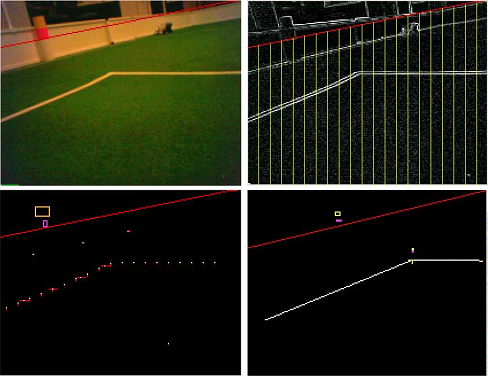
\includegraphics{RobinFig/linesfig.png} }
    \caption{Line detection steps. (top left) original image. (top right)Edge Classified image with vertical scan lines. (bottom left) the found line points. (bottom right) Final lines with the corner uniquely identified.}
    \label{fig:lines1}
    %\leavevmode
\end{center}
\end{figure}

For more details on the exact methods used please refer to the 2005 team report.